\documentclass{beamer}
\mode<presentation>
\usetheme{CambridgeUS}
\usepackage[russian]{babel}
\usepackage[utf8]{inputenc}
\usepackage[T2A]{fontenc}
\usepackage{sansmathaccent}

\usepackage{verbatim}
\usepackage{alltt}

\pdfmapfile{+sansmathaccent.map}
\title[Массивы]{Концепция типов данных. Массивы}
\author{Наумов Д.А., доц. каф. ИТГД}
\date[11.02.2019] {Алгоритмические языки и программирование, 2019}

\begin{document}

%ТИТУЛЬНЫЙ СЛАЙД
\begin{frame}
  \titlepage
\end{frame}
  
%СОДЕРЖАНИЕ ЛЕКЦИИ
\begin{frame}
  \frametitle{Содержание лекции}
  \tableofcontents  
\end{frame}
  
%РАЗДЕЛ 1
\section{Типы данных}

\subsection{Организация данных в программах}
\begin{frame}[t]
Программирование языке низкого уровня требует точного знания: 
\begin{itemize}
\item как данные представлены в виде последовательности битов;
\item какие машинные команды должны применяться для реализации требуемых операций.
\end{itemize}
Язык высокого уровня обеспечивает следующие возможности:
\begin{itemize}
\item на объекты данных ссылаются с помощью определенных пользователем имен, а не конкретных адресов памяти;
\item объекты данных связаны с типом, определяющим множество значений, которые могут приниматься объектами этого типа, и множество операций, которые могут применяться к объектам этого типа.
\end{itemize}
Хороший механизм типов является ключевым фактором при обеспечении
надежности языка программирования, что имеет первостепенную важность при программировании.
\end{frame} 

\subsection{Механизм типов данных}
\begin{frame}[fragile]
Тип данных специфицирует:
\begin{itemize}
\item структуру объектов;
\item область значений, которые могут принимать данные этого типа;
\item множество операций, применимых к данным этого типа. 
\end{itemize}
\begin{alltt}
1  var
2    i, j, k: integer;
3    n: longint;
(*  знак 0..1 bit, мантисса 39..40 bit, эспонента 8 bit  *)
4    b: real;  
5    c: char;
6  begin
7    j := i / 2;
8    n := succ(n);
9    c := chr(13);
10 end;
\end{alltt}
\end{frame}
   
\begin{frame}[c]
В общем случае в языке программирования должно быть \emph{множество предопределенных типов данных} и \emph{набор механизмов для спецификации типов}, определяемых пользователем.
\begin{block}{Типы данных}
\begin{enumerate}
\item простые;
	\begin{itemize}
	\item нет внутренней структуры;
	\item могут содержать лишь одно значение;
	\item доступные операции предопределены;	
	\end{itemize}
\item структурные
	\begin{itemize}
	\item состоят из других простых и (или) структурных типов;
	\item могут содержать составные значения;
	\item могут инкапсулировать поведение.	
	\end{itemize}
\end{enumerate}
\end{block}
\end{frame}   

\subsection{Слабая и сильная типизация}
\begin{frame}[fragile]
\begin{block}{Особенности слабой типизации}
\begin{itemize}
\item операция, которая может восприниматься машиной как корректная,
может быть некорректной на абстрактном уровне программы;
\begin{alltt}
1  var c: char;
2  c := 10;
\end{alltt}
\item для сохранения корректности предусмотрено выполнение операции преобразования типа;
\begin{alltt}
1  var x,y: real; 
2  var i,j,k: integer; 
3  i := x;
4  k := y - j;
\end{alltt}
\item увеличение гибкости, обеспечиваемое слабой типизацией, является слишком дорогой ценой за резкое уменьшение ясности программ и необходимость дополнительного контроля во время работы компилятора.	
\end{itemize}
\end{block}
\end{frame}   

\begin{frame}[fragile]
\begin{block}{Особенности сильной типизации}
\begin{itemize}
\item каждый объект обладает уникальным типом;
\item тип определяет множество значений и множество операций;
\item тип присваиваемого значения и тип объекта данных, которому производится присваивание, должны быть эквивалентны;
\item применяемая к объекту операция должна принадлежать множеству операций, определяемому типом объекта.
\end{itemize}
\begin{alltt}
1  var x: real;
2      i: integer;
3      b: boolean;
4      c: char;
5  i := 'A' (*разные типы в левой и правой частях*)
6  x := i;
7  i := i or 10; (*недопустимая операция*)
\end{alltt}
\end{block}
\end{frame}   

\subsection{Производные типы данных}
\begin{frame}[fragile]
На абстрактном уровне тип данных можно рассматривать как множество определенных свойств, являющихся общими для конкретного класса
объектов. 

\begin{alltt}
1  var age, total_age : integer;
2    i: integer;
3  begin
4    total_age := 0;
4    for i := 1 to 10 do begin
5      readln(age);
6      total_age := total_age + age;
7    end;
8    writeln(total_age);
9  end.

(* ошибочная строка *)      
      total_age := total_age + i;
\end{alltt}
\end{frame}   

\begin{frame}[fragile]
Преимущество сильной типизации: программисту разрешается определять при описании типа свои собственные типы. 

\begin{alltt}
1  type 
2    TAge = 0..200;
3    TIndex = 1..10;
4  var 
5    age, total_age : TAge;
2    i: TIndex;
3  begin
4    total_age := 0;
4    for i := 1 to 10 do begin
5      readln(age);
6      total_age := total_age + age;
7    end;
8    writeln(total_age);
9  end.
\end{alltt}
\end{frame}
   
\begin{frame}[fragile]
Имеются две различные основы для вычисления эквивалентности типов данных:
\begin{itemize}
\item структурная эквивалентность: два объекта принадлежат эквивалентным типам, если у них одинаковая структура;
\item именная эквивалентность: два объекта принадлежат эквивалентным типам, если они описаны с помощью одного и того же типа.
\end{itemize}

В языке Pascal принят принцип именной эквивалентности типов, устанавливающий, что два типа T1 и T2 эквивалентны, если выполняется одно из следующих условий:
\begin{itemize}
\item T1 и T2 — одно и то же имя типа;
\item Тип T2 описан с использованием типа T1 равенством вида type T2=T1; или последовательностью подобного вида равенств.
\end{itemize}
\begin{alltt}
1  type T1 = integer;
2    T3 = T1;
3    T2 = T3;
4    T4 = 1..10;
5    T5 = 1..10; 	
\end{alltt}
\end{frame}   

\subsection{Классификация типов данных в языке Pascal}
\begin{frame}
\begin{figure}[h]
\centering
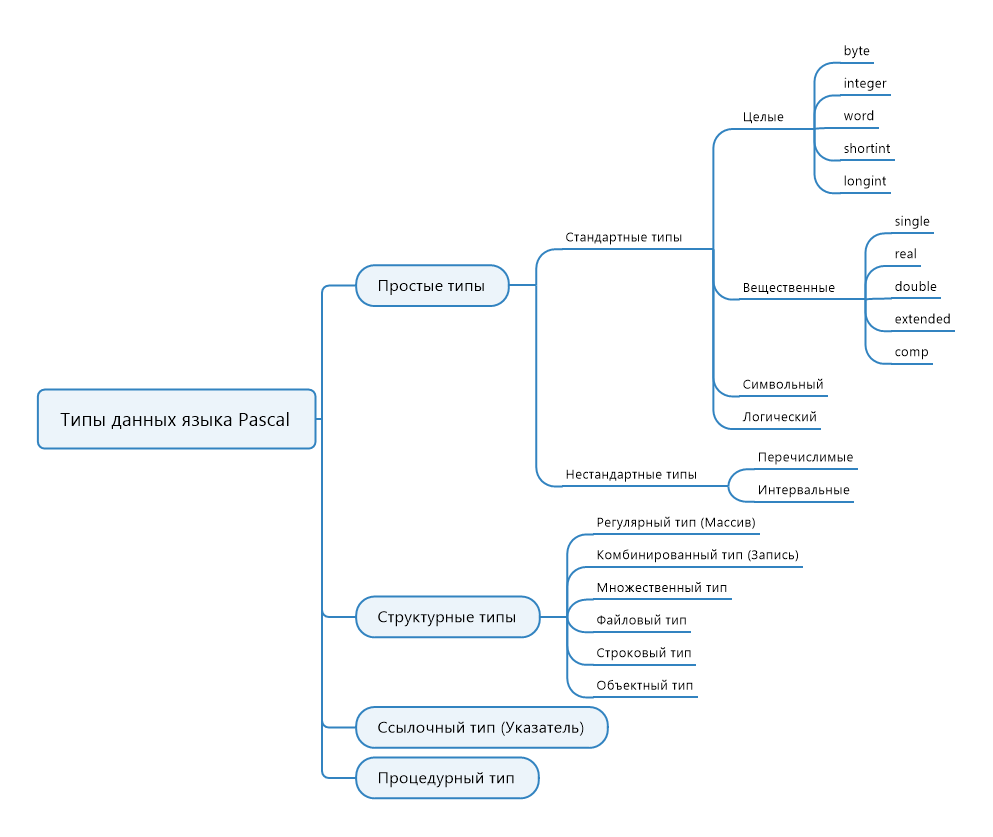
\includegraphics{images/tree_of_types.png}
\caption{Классификация типов языка Pascal}
\label{pic-tree-of-types}
\end{figure}
\end{frame} 

\begin{frame}[fragile]
\textbf{Перечисляемый тип} данных относится к нестандартным порядковым типам и определяется набором идентификаторов, с которыми могут совпадать значения переменных этого типа.
\begin{alltt}
1  type TDay = (MO, TU, WE, TH, FR, SA, SU);
2  var  D: TDay; 	
3  (* ORD (WE) = 2 *)
\end{alltt}
Максимальная мощность перечисляемого типа - 256 значений.
\begin{alltt}
(* типы эквивалентны по внутреннему представлению...*)
1  type TColors = (black, red, white );
2       TOrdenal=(one, two, three);
3       TDays=(monday, thesday, wednesday); 	
4  var  col: TColor; num: TOrdenal; day: TDays;
(* допустимые операторы присваивания *)
5  col := black; num := two; day := monday;
(* недопустимые операторы присваивания *)
6  col := two; day := black;
\end{alltt}
\end{frame}
   
\begin{frame}[fragile]
Для перечисляемых типов определены стандартные функции PRED, SUCC и ORD, имеющие тот же смысл, что и для стандартных скалярных типов.
\begin{alltt}
1  type TColors = (black, red, white);
2  (* SUCC(red) = white *)
3  (* PRED(red) = black *)
4  (* ORD(red) = 1 *)
\end{alltt}
\begin{itemize}
\item значения перечисляемого типа должны быть определены только идентификатором (именем);
\item нельзя присваивать переменной значение из описания другого типа;
\item недопустимо описание двух и более перечисляемых типов с совпадающими значениями;
\item нельзя значения перечисляемого типа использовать для ввода и вывода.
\end{itemize}
\begin{alltt}
1 type TColor1 = (red, yellow, blue);
2      TColor2 = (green, blue, gray);
\end{alltt}
\end{frame}   

\begin{frame}[fragile]
\textbf{Ограниченный тип данных} относится к нестандартным порядковыми
типам, образуется на основе порядковых типов, называемых базовыми,
путём ограничения диапазона значений этих типов заданием минимального и максимального значений.
\begin{alltt}
1  type TDay = (MO, TU, WE, TH, FR, SA, SU);
2       TNumber = 10..25;
3       TChars = 'c'..'x';
4       TWeekDays = SA..SU;
\end{alltt}
\begin{itemize}
\item базовым типом для создания ограниченного типа может быть любой
порядковый тип;
\item два символа ".." рассматриваются как один символ, поэтому между
ними не допустимы пробелы;
\item необходимо, чтобы левая граница диапазона не превышала его правую
границу.
\end{itemize}
\end{frame}

%РАЗДЕЛ 2
\section{Массив}
\subsection{Определение, описание, модель}

\begin{frame}[fragile]
\textbf{Массив} ~-- упорядоченный набор однотипных элементов (компонентов массива), доступ к которым осуществляется при помощи индекса.
Основные характеристики массива:
\begin{itemize}
\item размерность (одномерный, двухмерный и т.д.);
\item тип индексов;
\item тип элементов;
\end{itemize}
\begin{alltt}
(* Описание типа одномерного массива *)
1  type ИмяТипа = array[ТипыИндексов] of ТипЭлемента;
2  var ИмяПеременной1: ИмяТипа;
(* Описание переменной-массива *)
3  var ИмяПеременной2: array[ТипыИндексов] of ТипЭлемента;
\end{alltt}
\end{frame}

\begin{frame}[fragile]
Доступ к элементам массива осуществляется при помощи индексов. Тип индексов может быть любым порядковым типом:
\begin{itemize}
\item целым (byte, shortint, integer, word);
\item символьным (char);
\item логическим (boolean);
\item перечисляемым;
\item отрезковым.
\end{itemize}
\begin{alltt}
1 type
2    digit = array[0..9] of char; (*одномерный массив*)
(* двухмерный массив *)
3    matrix = array[byte, 'A'..'D'] of real;  
4 var
5    A, B : digit;
6    M1, M2 : matrix; 
(* трехмерный массив *)
7    Cube : array[1..5, 'A'..'H', boolean] of char; 
\end{alltt}
\end{frame}

\begin{frame}
Массивы могут использовать для представления списка или вектора (одномерный массив), матрицы (двумерный массив), и т.д. 
\begin{figure}[h]
\centering
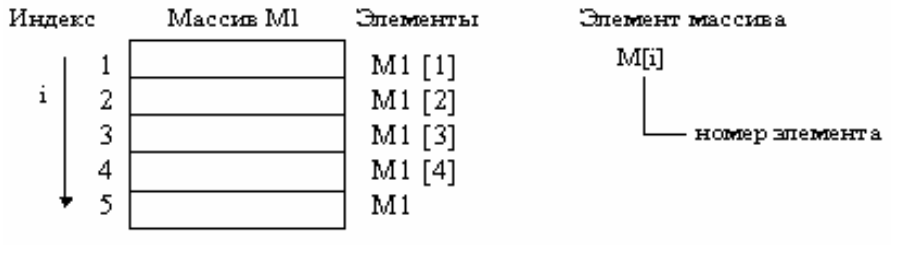
\includegraphics[scale=0.5]{images/one_index.png}
\caption{Одномерный массив}
\label{pic-one-index}
\end{figure}
\end{frame}

\begin{frame}
Массивы могут использовать для представления списка или вектора (одномерный массив), матрицы (двумерный массив), и т.д. 
\begin{figure}[h]
\centering
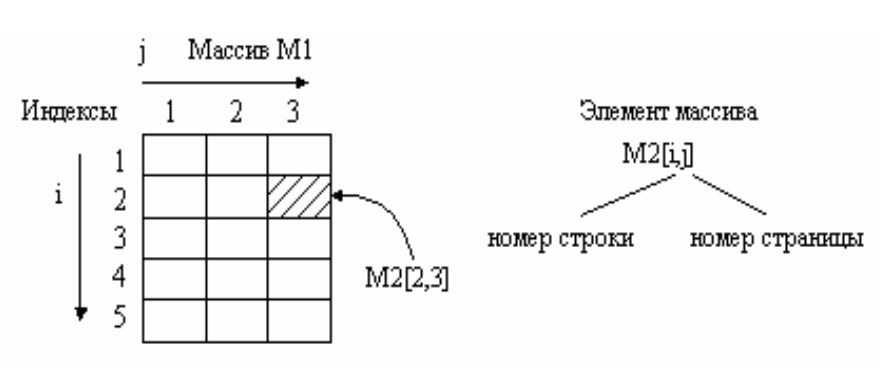
\includegraphics[scale=0.5]{images/two_index.png}
\caption{Двумерный массив}
\label{pic-two-index}
\end{figure}
\end{frame}

\subsection{Операция индексации}
\begin{frame}[fragile]
Доступ к отдельному элементу массива осуществляется при помощи операции индексации: указанием идентификатора массива, за которым в квадратных скобках указаны выражения, тип значения и количество которых соответствуют типам индексов.
\begin{alltt}
1 type Fam = (Ivanov, Petrov, Sidorov);
2   TMark = 2..5; 
3 var 
4   MarksAvg: array[Fam] of real;
5   Group741, Group748: array[1..30] of TMark;
6   i, j, k: integer;
\end{alltt}
К компонентам массива применимы операции и функции, допустимые для переменной базового типа. 
\begin{alltt}
1 i := 15; j := 20; k := 10;
2 MarksAvg[ Ivanov ] := 4.75;
3 Group741[i] := Group748[j - k];
(* допустимо при совпаднии типов индексов и элементов *)
4 Group748 := Group741; 
\end{alltt}
\end{frame}

\subsection{Типовые операции с массивом}
\begin{frame}
Ввод элементов одномерного массива при помощи цикла с параметром.
\begin{figure}[h]
\centering
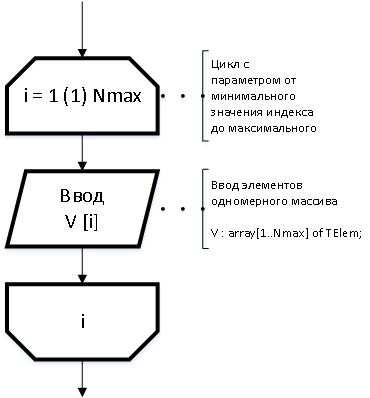
\includegraphics[scale=0.5]{images/array_input.png}
\caption{Ввод элементов одномерного массива}
\label{pic-input-one-index}
\end{figure}
\end{frame}

\begin{frame}
Ввод элементов одномерного массива при помощи цикла с параметром.
\begin{figure}[h]
\centering
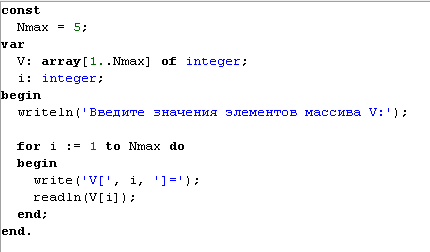
\includegraphics[scale=1.0]{images/array_input_code_one.png}
\caption{Ввод элементов одномерного массива}
\label{pic-input-one-index-code}
\end{figure}
\end{frame}

\begin{frame}
Ввод элементов двумерного массива при помощи вложенный циклов.
\begin{figure}[h]
\centering
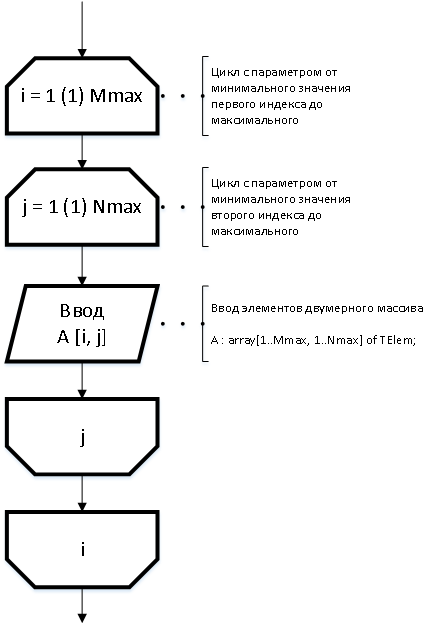
\includegraphics[scale=0.45]{images/array_input_two.png}
\caption{Ввод элементов двумерного массива}
\label{pic-input-two-index}
\end{figure}
\end{frame}

\begin{frame}
Ввод элементов двумерного массива при помощи вложенных циклов.
\begin{figure}[h]
\centering
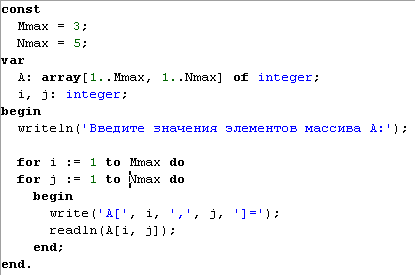
\includegraphics[scale=1.0]{images/array_input_code_two.png}
\caption{Ввод элементов двумерного массива}
\label{pic-input-two-index-code}
\end{figure}
\end{frame}

\begin{frame}
Вывод элементов одномерного массива.
\begin{figure}[h]
\centering
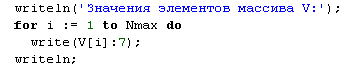
\includegraphics[scale=1.0]{images/array_output_code_one.png}
\caption{Вывод элементов одномерного массива}
\label{pic-output-code-one}
\end{figure}

Вывод элементов двумерного массива.
\begin{figure}[h]
\centering
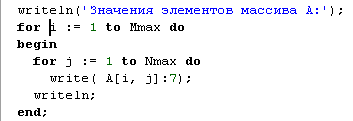
\includegraphics[scale=1.0]{images/array_output_code.png}
\caption{Вывод элементов двумерного массива}
\label{pic-output-code-two}
\end{figure}
\end{frame}

\begin{frame}
В одномерном массиве М, состоящем из N целых чисел, найти элементы, значения которых равны заданному числу K.
\begin{figure}[h]
\centering
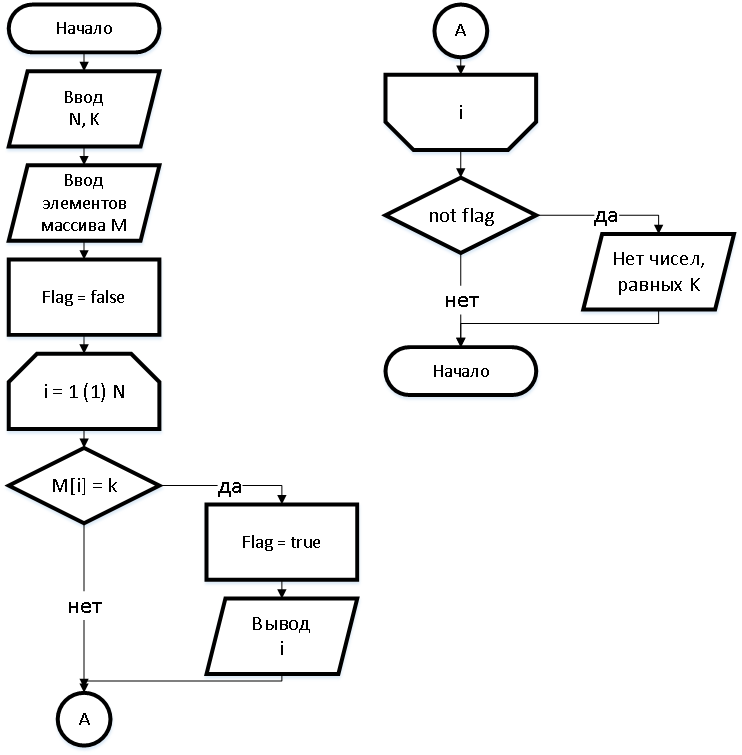
\includegraphics[scale=0.35]{images/array_search.png}
\caption{Поиск элементов в одномерном массиве}
\label{pic-search}
\end{figure}
\end{frame}

\begin{frame}
В одномерном массиве М, состоящем из N целых чисел, найти элементы, значения которых равны заданному числу K.
\begin{figure}[h]
\centering
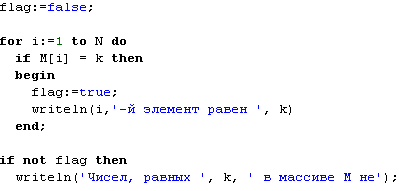
\includegraphics[scale=1.0]{images/array_search_code.png}
\label{pic-search-code}
\end{figure}
\end{frame}

\begin{frame}
В одномерном массиве М, состоящем из N целых чисел, найти минимальное значение элемента.
\begin{figure}[h]
\centering
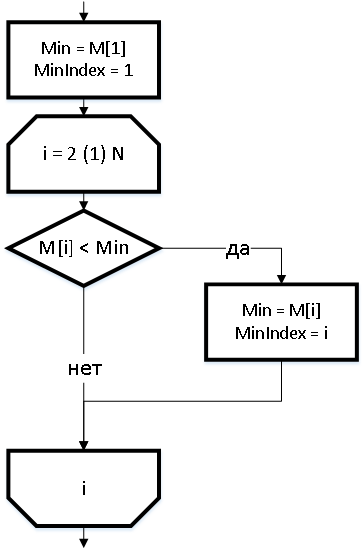
\includegraphics[scale=0.35]{images/array_min.png}
\caption{Поиск минимального элемента в одномерном массиве}
\label{pic-search}
\end{figure}
\end{frame}

\begin{frame}
В одномерном массиве М, состоящем из N целых чисел, найти минимальное значение элемента.
\begin{figure}[h]
\centering
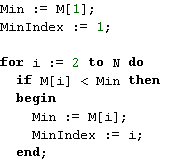
\includegraphics[scale=1.0]{images/array_min_code.png}
\label{pic-search-code}
\end{figure}
\end{frame}

\begin{frame}
Для обмена значениями двух элементов массива необходимо использовать вспомогательную переменную для временного хранения одного из элементов.
\begin{figure}[h]
\centering
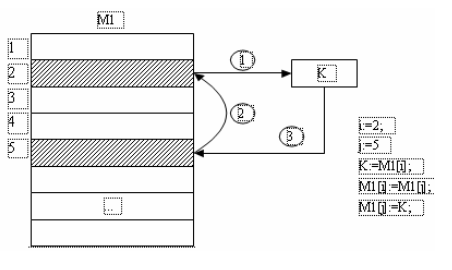
\includegraphics[scale=0.8]{images/array_swap.png}
\label{pic-search-swap}
\end{figure}
\end{frame}

\begin{frame}
Типовой задачей является сортировка элементов массива.
\begin{figure}[h]
\centering
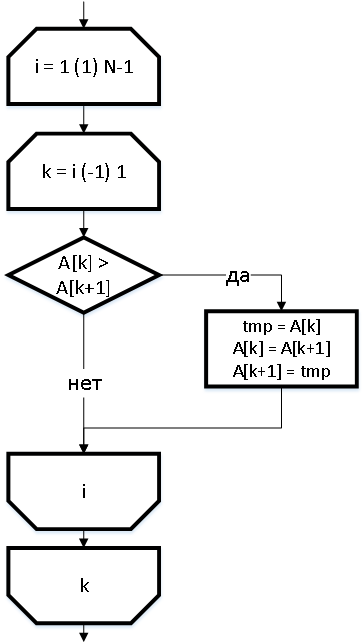
\includegraphics[scale=0.4]{images/array_sort.png}
\label{pic-sort}
\end{figure}
\end{frame}

\begin{frame}
Фрагмент кода для сортировки методом "пузырька".
\begin{figure}[h]
\centering
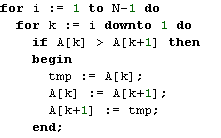
\includegraphics[scale=1.0]{images/array_sort_code.png}
\label{pic-sort}
\end{figure}
\end{frame}

\begin{frame}[fragile]
Объявление констант типа массив позволяет задать значение компонент неизменяемого массива.
\begin{alltt}
1  Type Status = (Active, Passive, Waiting); 
2    StatusMap = Array [Status] Of String[7];
3  Const StatStr : StatusMap = ('Active', 'Passive', 'Waiting');
\end{alltt}
Упакованные константы со строковым типом (символьные массивы) могут быть определены и как одиночные символы, и как строки.
\begin{alltt}
4  Const Digits1 : array [0..9] Of Char 
         = ('0', '1', '2', '3', '4', '5','6', '7', '8', '9'); 
5  Const Digits2 : array [0..9] Of Char = '0123456789';
\end{alltt}
Константы - многомерные массивы определяются заключением констант каждой размерности в отдельные наборы круглых скобок, разделенные запятыми.
\begin{alltt}
6  Type Cube = array[0..1, 0..1, 0..1] Of Integer;
7  Const Array_Maze : cube = 
     (((0, 1), (2, 3)), ((4, 5), (6, 7)));
\end{alltt}
\end{frame}
   
\section*{Литература}
\begin{frame}   
\begin{enumerate}
\item Алгоритмические языки и основы программирования: Учебное пособие / В.Д.Былкин, Ю.В Блинков, Т.А. Глебова, В.В. Пикулин / Под общ ред. проф. А.Н.Кошева. - Пенза: ПГУAC, 2004. - 280 с. ISBN 5-9282-022J-0
\end{enumerate}
\end{frame}   

\end{document}
